\subsection{Control Loop (CL)}
\label{subsec:control_loop}

The \acrfull{cl} act as the brain of the clock, adjusting dynamically various parameters inside the \acrshort{csac} architecture to optimize stability and output frequency accuracy.
To do so, multiple servo loops based on PI\footnote{Proportional Integral} controllers are implemented to control specific areas and properties of different components. \acrshort{cl} takes as input the signal coming from the \acrfull{pp} and other sampled quantities coming from a network of sensors that are used to monitor the state of the clock (e.g., temperature sensors, magnetic field sensors, etc.)

\begin{figure}[H]
    \centering
    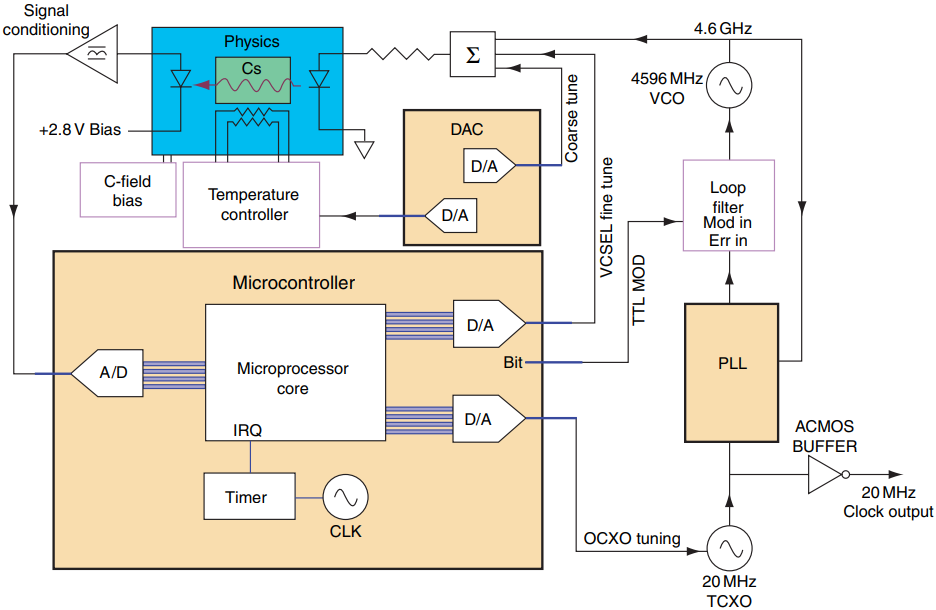
\includegraphics[width=.7\textwidth, max width=\linewidth]{img/control-loop.png}
    \caption{Control Loops block diagram for a CPT-based architecture (note the presence of the VCSEL). Source \cite{Knappe}.}
    \label{fig:control-loop}
\end{figure}

In Figure \ref{fig:control-loop} some key components are highlighted, such as microcontroller, converters (DAC and ADC), and PLL (Phase-Locked Loop) that are crucial for the correct functioning of the \acrshort{cl}.
In particular, the PLL is responsible for keeping in phase the \acrshort{lo} (indicated by the label "TCXO" in the bottom right) with the \acrshort{fs}, minimizing the phase noise and the frequency drift between the two components.

In a regular architecture, at least four servo loops are implemented to target different parameters.


\paragraph{Local Oscillator frequency servo loops}

The most important task of the \acrshort{cl} is the discipline of the \acrfull{lo} frequency to the desired value, locking it to the atomic resonance frequency or one of its multiple harmonics.

To achieve this, the \acrshort{cl} receives the output signal from the \acrshort{pp} and generate a feedback voltage signal that is sent to the \acrshort{lo} group.
Here, it's converted in a temperature variation of the crystal in order to modify its mechanical properties, thus adjusting the output frequency.

With reference to Figure \ref{fig:control-loop}, we can see this control line in the bottom right corner of the image, associated with the label "OCXO tuning", going from the microcontroller unit to the \acrshort{lo} group.

It has to be noted that the \acrshort{lo} has a much slower dynamics with respect to the electrical one provided by the microcontroller.
This causes an unavoidable delay over the feedback loop action and the actual effect on the \acrshort{lo} output frequency.


\paragraph{Laser frequency servo loops}

In case of the use of VCSEL as the excitation source, the \acrshort{cl} is also responsible for the control and tuning of its frequency that can be affected by external factors such as temperature variations or electrical/magnetic disturbances.

The diode laser is controlled by the summation of three different signal (see Figure \ref{fig:control-loop}), that are the coarse tune, the fine tune, and the \acrshort{fs} output.

In particular, the coarse tune signal is independent of any state of the clock and doesn't vary during the operation time.
The fine tune instead, is generated by the microcontroller and is used to compensate the environmental effects that cause a drift in the frequency of the excitation source.
Finally, the \acrshort{fs} output is added in order to permit the \acrshort{pp} to understand if the \acrshort{lo} is locked to the atomic resonance frequency.


\paragraph{Laser and cell temperature servo loops}

Maintaining constant temperatures for the laser and the reference cell within the \acrshort{pp} is another job of the \acrshort{cl}.

As we will see in the next section (Section \ref{sec:performances_and_limitations}), the temperature of these two components are crucial for the performances of the clock and should be maintained at a constant value during the operation time.

To do so, the feedback loop modify the temperature based on the signal coming from a network of thermocouple sensors that are placed near the targets.
Notice how, depending on the specific architecture of the clock, the \acrshort{cl} can act on the temperature of the two components independently or together.

In this way, the \acrshort{cl} ensures that both the excitation source and the atomic resonance frequencies are not affected by temperature variations, improving the photons coupling effectiveness.


\paragraph{Other servo loops}

In addition, other control loops can be implemented to target other parameters that might affect the performances of the clock.

Among these, one of particular importance is the servo used to shield or more in general control the magnetic field surrounding the \acrshort{pp}.
Again, with reference to Figure \ref{fig:control-loop}, we can recognize this control line in the bottom left corner of the "Physics" package block, associated with the label "C-field bias".

This control loop is used to maintain a zero or a constant value of the magnetic field inside the \acrshort{pp}, ensuring a precise and predictable behavior of the atomic resonance frequency that otherwise might suffer from frequency shifts (Zeeman and Stark effects, see Section \ref{sec:performances_and_limitations}).
